% 第四章 项目市场分析
\section{项目市场分析}

\subsection{市场环境分析}

\subsubsection{PEST分析}

\textbf{Political(政治环境)}:国家层面高度重视数字政府和智慧城市建设,《深化智慧城市发展推进全域数字化转型行动计划》明确提出到 2027年底建成50个以上全域数字化转型城市的目标。河南省设立30亿元人工智能产业基金,对通过国家生成式AI模型备案的企业给予100万元资金支持。舆情管理已纳入城市治理体系,各级政府对舆情监测能力建设需求明确。

\textbf{Economic(经济环境)}:中国舆情监测市场2025年预计突破72.4亿元,年增速高达26.4\%\textsuperscript{[6]},远超全球平均水平。地级市、县域市场存在大量空白,主流产品年费动辄3-100万元,中小客户难以承担,形成显著的价格缝隙市场。AI技术的成熟大幅降低了舆情分析成本,云服务的普及使得轻量化SaaS部署成为可能,中小企业的舆情监测需求正在加速释放。

\textbf{Social(社会环境)}:社交媒体用户规模持续增长,我国网民规模已超过10亿,舆情传播速度显著加快。短视频、直播已成为舆情爆发的主渠道,传统的文字监测手段难以全面覆盖。公众对政府信息透明度和响应速度要求不断提高,企业品牌声誉意识增强,危机公关和品牌维护需求持续上升。

\textbf{Technological(技术环境)}:大语言模型技术已趋成熟,2025年主流系统情感识别准确率普遍超过90\%\textsuperscript{[7]}。多模态分析能力大幅提升,支持图片、视频、音频等多种内容形式的解析。3D可视化技术已广泛普及,WebGL兼容性覆盖98\%以上现代浏览器。AI 3D生成技术快速兴起,秒级模型生成已成为现实,为舆情场景还原提供了技术基础。

\begin{figure}[H]
\centering
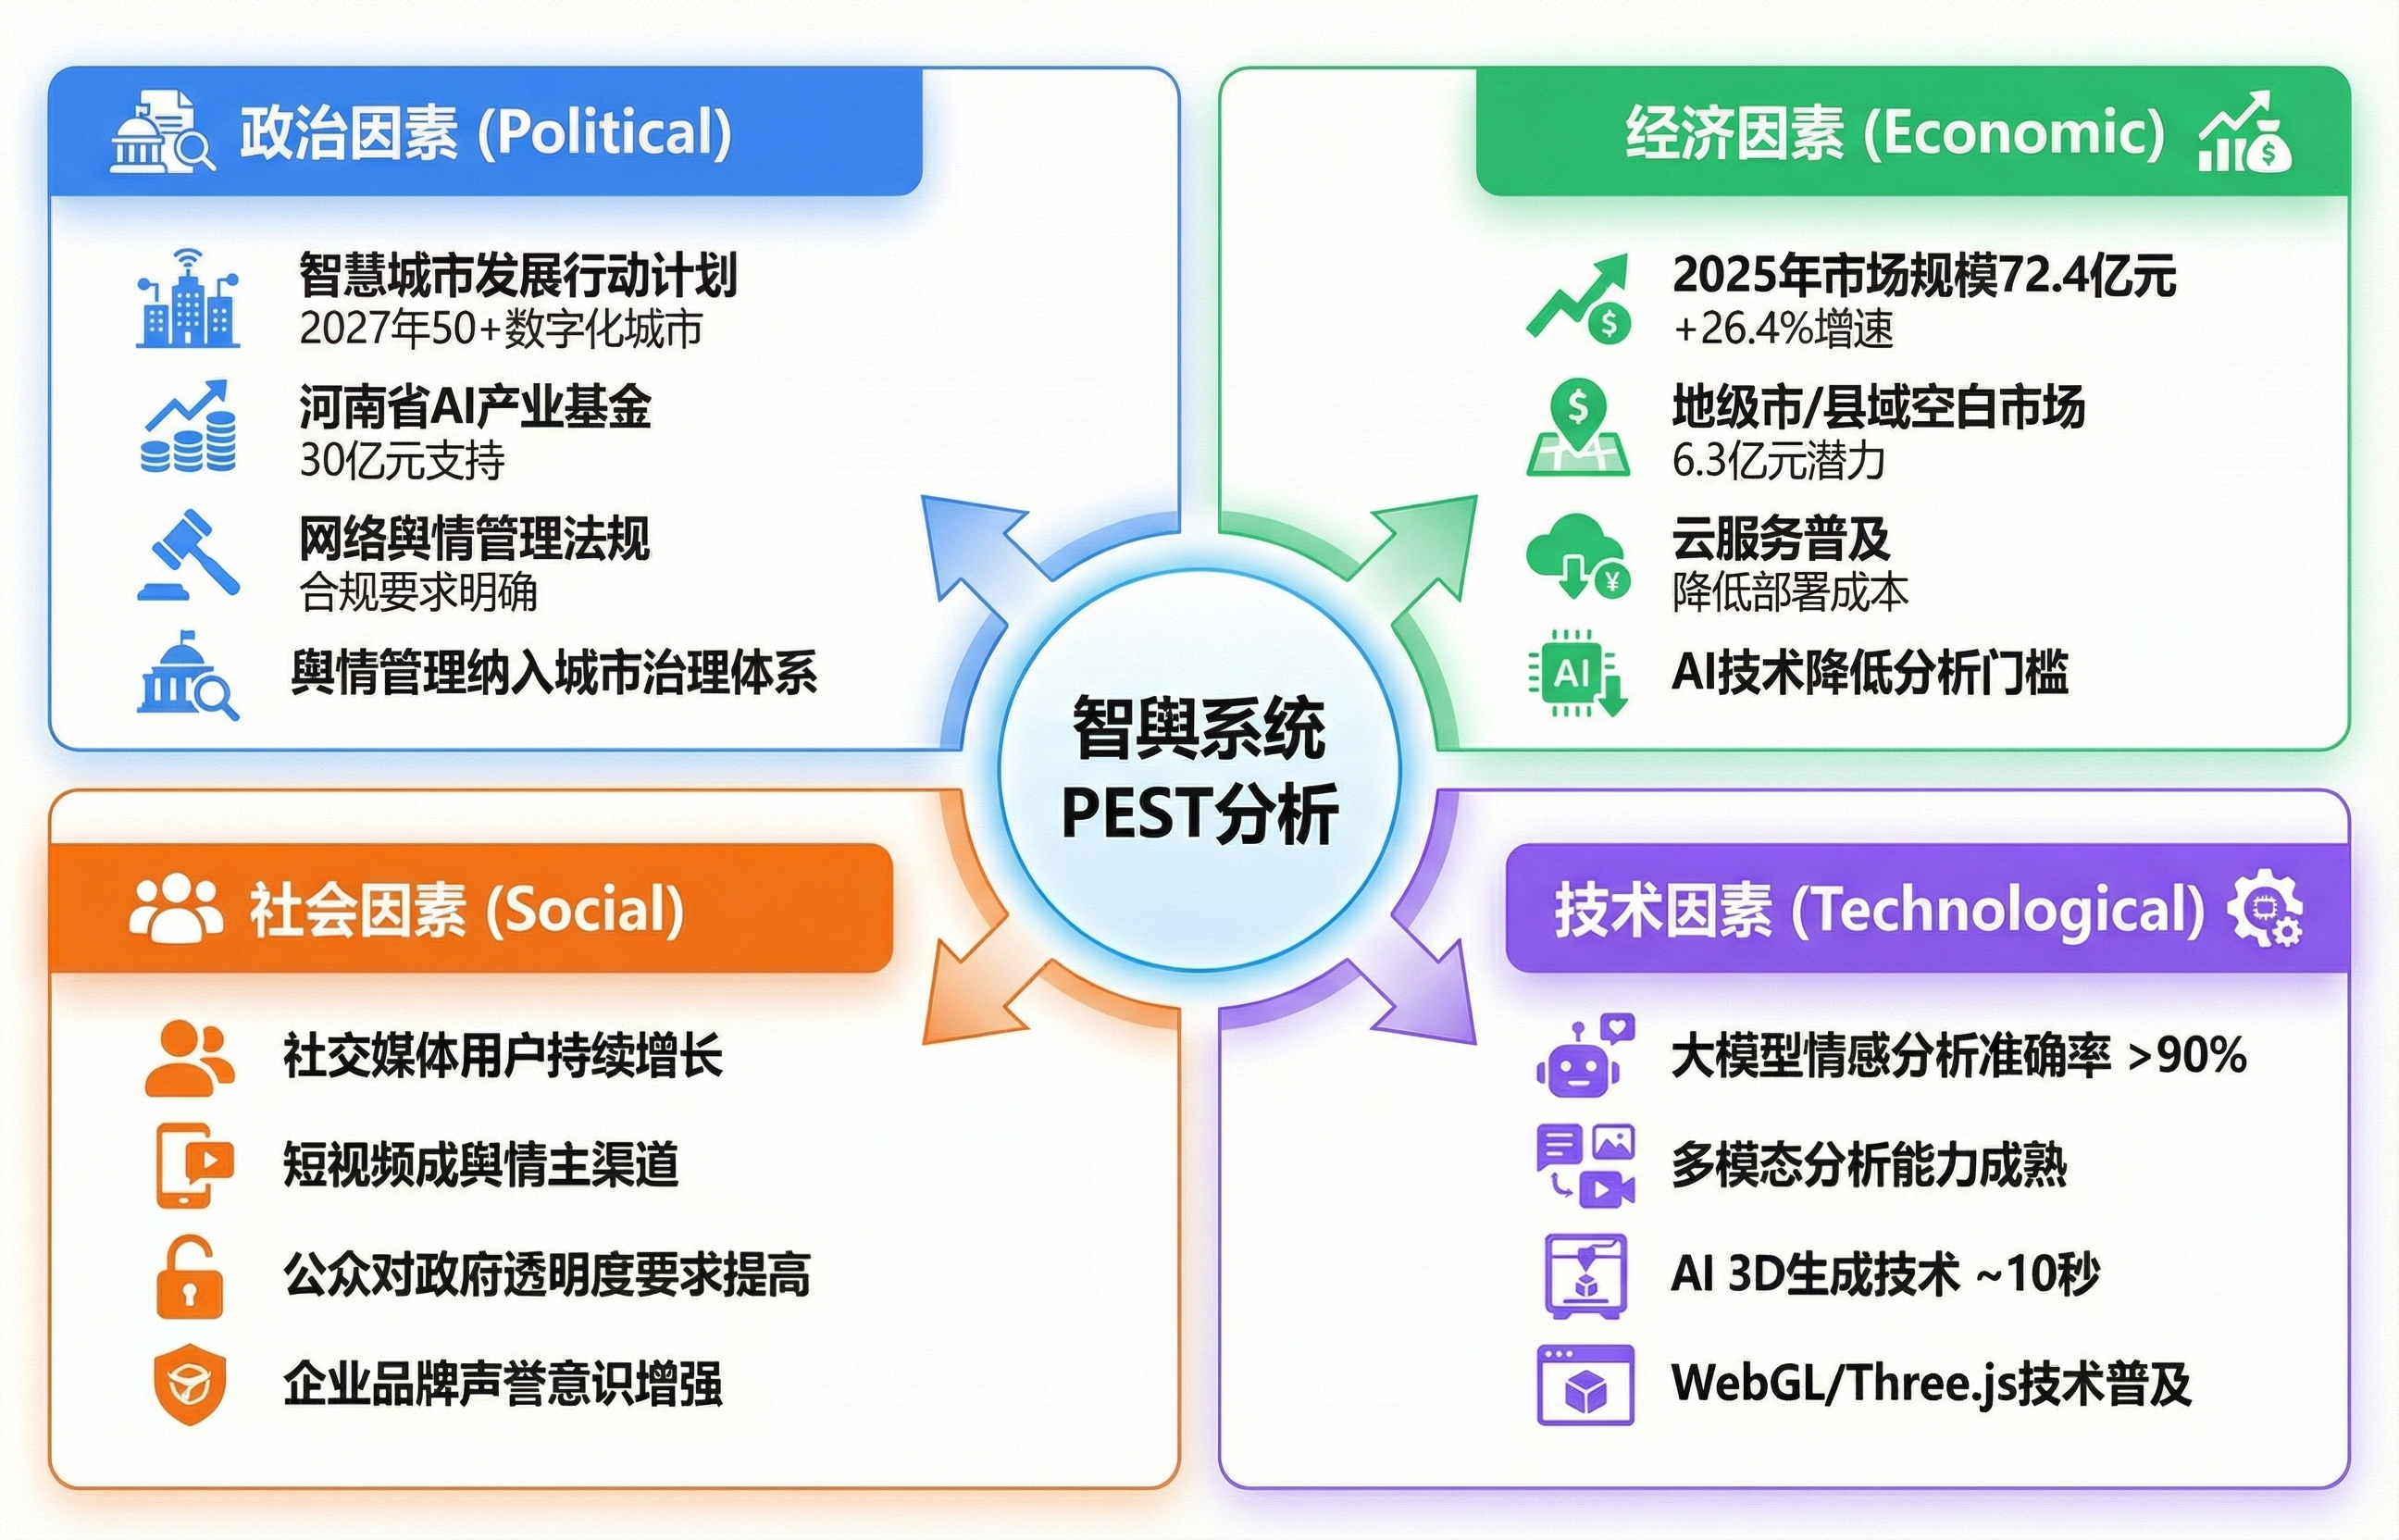
\includegraphics[width=0.85\textwidth]{../picture/fig14_PEST.png}
\caption{PEST分析四象限图}
\end{figure}

\subsubsection{行业现状}

\textbf{市场格局}

中国舆情监测市场呈现"一超多强"格局。\textbf{第一梯队}以新浪舆情通(蜜度)为代表,综合评分96.8分,稳居行业榜首,具备数据源全面、AI分析能力强等优势。\textbf{第二梯队}包括人民网舆情、蚁坊软件(鹰眼)、清博智能等,各具特色,分别在政务渠道、多语种支持、学术研究等方面具备优势。\textbf{第三梯队}包括慧科讯业、拓尔思、TOOM等企业,在细分领域有一定竞争力。

\textbf{竞争态势}:头部企业占据市场主导地位,但存在明显的机会窗口。首先是\textbf{价格门槛高},主流产品年费3-100万元,中小客户望而却步。其次是\textbf{功能过剩},大多数客户仅需基础监测和分析功能,高端功能利用率较低。再次是\textbf{下沉市场覆盖不足},地级市、县域等基层市场缺乏适配产品。最后是\textbf{创新空间大},3D可视化、AI场景生成、决策模拟等方向尚未被充分开发,为新进入者提供了差异化竞争的机会。

\subsection{项目市场趋势}

\subsubsection{市场规模}

\textbf{全球市场}:2024年规模23.15亿美元,2031年预测40.50亿美元,年复合增长率8.1\%\textsuperscript{[5]}。

\textbf{中国市场}:2024年规模110亿元人民币,年复合增长率15-26\%。

\textbf{地级市/县域市场}:全国共有地级市293个、县级行政区2844个。假设其中10\%具有舆情监测需求,平均客单价2万元/年,则潜在市场规模为:
\[
S = (293 + 2844) \times 10\% \times 2 \approx 627 \text{(万元)} \approx 6.3 \text{(亿元)}
\]
这是一个被头部企业忽视的巨大市场,也是智舆系统重点突破的目标市场。

\begin{figure}[H]
\centering
\includegraphics[width=0.9\textwidth]{../picture/fig15_market_forecast.png}
\caption{舆情监测市场规模增长预测图(2024-2031)}
\end{figure}

\subsubsection{增长驱动因素}

舆情监测市场增长受四大因素驱动。\textbf{政策推动}方面,智慧城市、数字政府建设加速推进,各级政府对舆情监测能力建设的重视程度持续提升。\textbf{技术进步}方面,AI大模型技术的成熟大幅降低了舆情分析的技术门槛和成本。\textbf{需求释放}方面,中小企业和基层政府的舆情监测意识逐步觉醒,市场需求加速释放。\textbf{场景拓展}方面,舆情监测应用从传统的政务管理领域向企业品牌维护、个人影响力管理等新场景延伸。

\subsection{目标市场}

\subsubsection{目标用户画像}

\textbf{核心用户群:地级市政府部门}

\begin{table}[H]
\centering
\caption{核心用户画像}
\begin{tabular}{L{3cm}L{10cm}}
\toprule
\textbf{特征维度} & \textbf{描述} \\
\midrule
机构类型 & 应急管理局、网信办、公安局、宣传部等 \\
预算范围 & 5-20万元/年 \\
核心需求 & 舆情监测、预警通知、分析报告 \\
痛点 & 技术人才缺乏、预算有限、现有工具不适配 \\
决策因素 & 价格、易用性、本地化服务 \\
\bottomrule
\end{tabular}
\end{table}

\textbf{拓展用户群:地方企业}

\begin{table}[H]
\centering
\caption{拓展用户画像}
\begin{tabular}{L{3cm}L{10cm}}
\toprule
\textbf{特征维度} & \textbf{描述} \\
\midrule
企业类型 & 本地品牌企业、餐饮连锁、房地产等 \\
预算范围 & 1-5万元/年 \\
核心需求 & 品牌监测、竞品分析、危机预警 \\
痛点 & 专业工具太贵、功能太复杂 \\
决策因素 & 性价比、操作简便 \\
\bottomrule
\end{tabular}
\end{table}

\subsubsection{市场细分}

\begin{table}[H]
\centering
\caption{市场细分分析}
\begin{tabular}{L{2.5cm}C{2cm}C{2cm}C{2cm}C{2cm}}
\toprule
\textbf{细分市场} & \textbf{市场规模} & \textbf{竞争强度} & \textbf{进入难度} & \textbf{优先级} \\
\midrule
信阳本地 & 小 & 低 & 低 & 高 \\
河南省内 & 中 & 中 & 中 & 中 \\
全国地级市 & 大 & 中 & 高 & 低(远期) \\
\bottomrule
\end{tabular}
\end{table}

\subsection{市场调查及分析}

\subsubsection{用户需求调研}

\textbf{政府部门需求}:$7\times24$小时不间断全网监测、多渠道预警、舆情分析功能、专项服务保障。

\textbf{企业用户需求}:实时监测品牌关键词、I级危机1小时内响应、竞品动态监测、定期舆情报告。

\subsubsection{竞品分析}

\begin{table}[H]
\centering
\caption{主要竞品对比}
\begin{tabular}{L{2.5cm}C{2cm}L{2.5cm}L{2.5cm}L{2.5cm}}
\toprule
\textbf{产品} & \textbf{评分} & \textbf{价格区间} & \textbf{核心优势} & \textbf{主要不足} \\
\midrule
新浪舆情通 & 96.8 & 3-25万/年 & 数据全、AI强 & 价格高 \\
人民网舆情 & 92.3 & 5-50万/年 & 权威背书 & 定制化程度高 \\
鹰眼速读网 & 89.7 & 3-30万/年 & 多语种 & 功能复杂 \\
清博舆情 & 87.5 & 2-20万/年 & 学术支撑 & 可视化一般 \\
\bottomrule
\end{tabular}
\end{table}

\textbf{智舆系统竞争定位}:差异化定位聚焦下沉市场,提供轻量化、低成本方案;3D可视化、AI生成、决策模拟形成差异化壁垒;立足信阳,深耕本地需求。

\begin{figure}[H]
\centering
\includegraphics[width=0.8\textwidth]{../picture/fig16.png}
\caption{竞品功能对比雷达图}
\end{figure}
